\documentclass[11pt]{article}

\usepackage{geometry}
% make full use of A4 papers
\geometry{margin=1.5cm, vmargin={0pt,1cm}}
\setlength{\topmargin}{-1cm}
\setlength{\paperheight}{29.7cm}
\setlength{\textheight}{25.1cm}
\usepackage[BoldFont,SlantFont,CJKchecksingle]{xeCJK}%CJKsetspaces
%\setCJKmainfont[BoldFont=SimHei]{SimSun}
%\setCJKmonofont{SimSun}% 设置缺省中文字体
\usepackage{indentfirst}
\setlength{\parindent}{2em}%段首缩进
\usepackage{setspace}
% \setlength{\baselineskip}{25pt}
\linespread{1.25}
% auto adjust the marginals
\usepackage{marginfix}
\usepackage{amsfonts}
\usepackage{amsmath}
\usepackage{bm}
\usepackage{amssymb}
\usepackage{amsthm}
\usepackage{CJKutf8}   % for Chinese characters
\usepackage{enumerate}
\usepackage{fancyhdr}
\usepackage{graphicx}  % for figures
\usepackage{layout}
\usepackage{mathrsfs}  
\usepackage{multicol}  % multiple columns to reduce number of pages
%\usepackage{natbib}
\usepackage{subfigure}
\usepackage{tcolorbox}
\usepackage{tikz-cd}
\usepackage{extarrows}
\usepackage{float}
\usepackage{diagbox}
\usepackage[backend=biber,style=gb7714-2015]{biblatex}
\addbibresource[location=local]{bib/3Dmars.bib}

%------------------
% common commands %
%------------------
% differentiation
\newcommand{\aff}{\mathrm{aff}}
\newcommand{\conv}{\mathrm{conv}}
\newcommand{\VertSet}{\mathrm{Vert}}
\newcommand{\Star}{\mathrm{st}}
\newcommand{\gen}[1]{\left\langle #1 \right\rangle}
\newcommand{\dif}{\mathrm{d}}
\newcommand{\difPx}[1]{\frac{\partial #1}{\partial x}}
\newcommand{\difPy}[1]{\frac{\partial #1}{\partial y}}
\newcommand{\Dim}{\mathrm{D}}
\newcommand{\avg}[1]{\left\langle #1 \right\rangle}
\newcommand{\sgn}{\mathrm{sgn}}
\newcommand{\Span}{\mathrm{span}}
\newcommand{\dom}{\mathrm{dom}}
\newcommand{\Arity}{\mathrm{arity}}
\newcommand{\Int}{\mathrm{Int}}
\newcommand{\Ext}{\mathrm{Ext}}
\newcommand{\Cl}{\mathrm{Cl}}
\newcommand{\Fr}{\mathrm{Fr}}
% group is generated by
\newcommand{\grb}[1]{\left\langle #1 \right\rangle}
% rank
\newcommand{\rank}{\mathrm{rank}}
\newcommand{\Iden}{\mathrm{Id}}
\newcommand{\Obj}[1]{\mathrm{obj}\,{\mathscr #1}}
\newcommand{\Hom}{\mathrm{Hom}}

% this environment is for solutions of examples and exercises
\newenvironment{solution}%
{\noindent\textbf{Solution.}}%
{\qedhere}

%the following command is for disabling environments
%  so that their contents do not show up in the pdf.
\makeatletter
\newcommand{\voidenvironment}[1]{%
  \expandafter\providecommand\csname env@#1@save@env\endcsname{}%
  \expandafter\providecommand\csname env@#1@process\endcsname{}%
  \@ifundefined{#1}{}{\RenewEnviron{#1}{}}%
}
\makeatother

%---------------------------------------------
% commands specifically for complex analysis %
%---------------------------------------------
% complex conjugate
\newcommand{\ccg}[1]{\overline{#1}}
% the imaginary unit
\newcommand{\ii}{\mathbf{i}}
%\newcommand{\ii}{\boldsymbol{i}}
% the real part
\newcommand{\Rez}{\mathrm{Re}\,}
% the imaginary part
\newcommand{\Imz}{\mathrm{Im}\,}
% punctured complex plane
\newcommand{\pcp}{\mathbb{C}^{\bullet}}
% the principle branch of the logarithm
\newcommand{\Log}{\mathrm{Log}}
% the principle value of a nonzero complex number
\newcommand{\Arg}{\mathrm{Arg}}
\newcommand{\Null}{\mathrm{null}\,}
\newcommand{\Range}{\mathrm{range}\,}
\newcommand{\Ker}{\mathrm{ker}}
\newcommand{\Iso}{\mathrm{Iso}}
\newcommand{\Aut}{\mathrm{Aut}}
\newcommand{\ord}{\mathrm{ord}}
\newcommand{\Res}{\mathrm{Res}}
%\newcommand{\GL2R}{\mathrm{GL}(2,\mathbb{R})}
\newcommand{\GL}{\mathrm{GL}}
\newcommand{\SL}{\mathrm{SL}}
\newcommand{\Dist}[2]{\left|{#1}-{#2}\right|}



%----------------------------------------
% theorem and theorem-like environments %
%----------------------------------------
% \numberwithin{equation}{chapter}
% \theoremstyle{definition}

% \newtheorem{thm}{Theorem}[chapter]
% \newtheorem{axm}[thm]{Axiom}
% \newtheorem{alg}[thm]{Algorithm}
% \newtheorem{asm}[thm]{Assumption}
% \newtheorem{defn}[thm]{Definition}
% \newtheorem{frm}[thm]{Formula}
% \newtheorem{prop}[thm]{Proposition}
% \newtheorem{qst}[thm]{Question}
% \newtheorem{rul}[thm]{Rule}
% \newtheorem{coro}[thm]{Corollary}
% \newtheorem{lem}[thm]{Lemma}
% \newtheorem{exm}{Example}[chapter]
% \newtheorem{rem}{Remark}[chapter]
% \newtheorem{exc}[exm]{Exercise}
% \newtheorem{ntn}{Notation}


%----------------------
% the end of preamble %
% ----------------------


\begin{document}
% \begin{CJK*}{UTF8}{gkai}
% 		\CJKindent
 % \makeatletter %将文献引用作为上标出现,增加括号,
 % \def\@cite#1#2{\textsuperscript{[{#1\if@tempswa , #2\fi}]}}

 % \makeatother
 \theoremstyle{definition}%amsthm 宏包 标签正体,内容正体
 \newtheorem{thm}{{定理}}
 \newtheorem{lem}[thm]{{引理}}
 \newtheorem{defn}[thm]{{定义}}
\newtheorem{prop}[thm]{{性质}}
 \newtheorem{cor}[thm]{{推论}}
 \newtheorem{nota}[thm]{{记号}}
 \newtheorem{exm}{{例}}
 \newtheorem{rem}[exm]{{注}}
 \newtheorem*{pro}{证明}

\title{三维曲率流算法稳定性数值测试}
\author{金鹏炜}
\date{}
\maketitle

\section{局部坐标系的选取方案}
\indent
在选取局部坐标系时,我们有两种方案,如图\ref{fig:局部坐标系的选取}所示,在计算球面上一点$\bm{X}_0$的曲率流右端项时,方案一选取$\bm{X}_0$及其邻近两示踪点$\bm{X}_1,\bm{X}_2$构成的平面为投影平面,即红色三角形所在平面;方案二先根据方案一构造局部坐标系,计算$\bm{X}_0$处的单位外法向量$\vec{\bm{n}}$,再沿$\vec{\bm{n}}$投影构造局部坐标系,即蓝色平面为投影平面。
\begin{figure}[htbp]
\centering
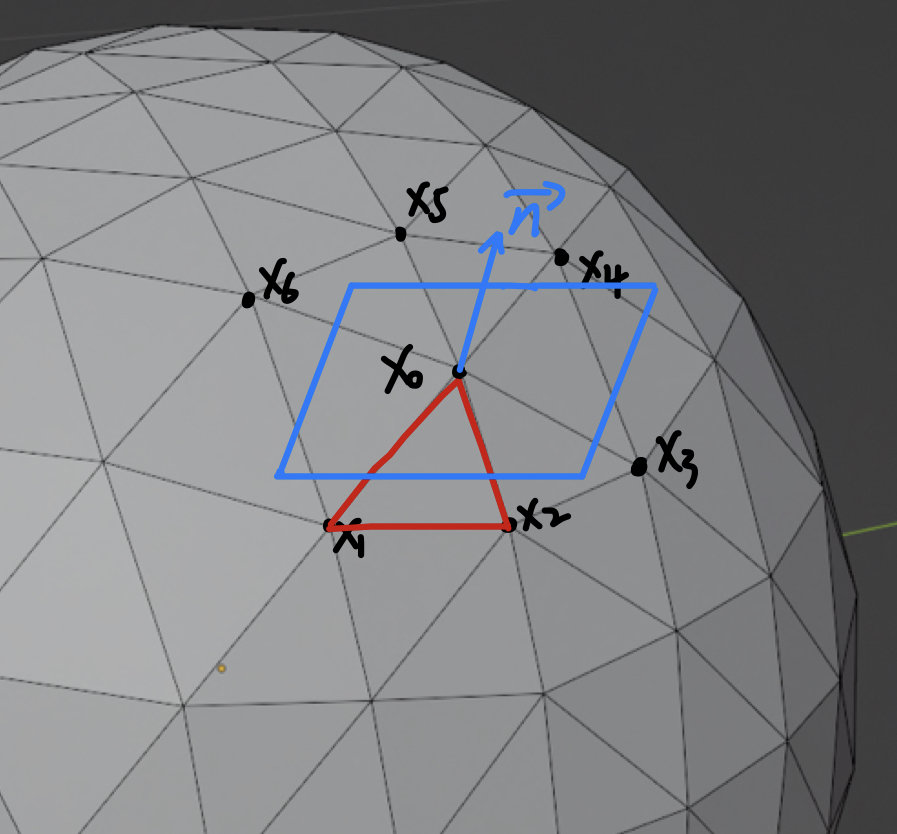
\includegraphics[scale=0.2]{fig/局部坐标系选取.jpg}
\caption{局部坐标系的选取}
\label{fig:局部坐标系的选取}
\end{figure}
\section{二阶方法数值测试}
\begin{rem}
  一时疏忽,忘记输出最后时刻的最大正实特征值,导致表\ref{tab:二阶方法非法向投影最大正实特征值}、表\ref{tab:二阶方法法向投影最大正实特征值}和表\ref{tab:四阶方法非法向投影最大正实特征值}少了一列,但并不影响分析。
\end{rem}
\begin{table}[H]
  \centering
  \begin{tabular}{c|ccccc}
    \hline
    $h_L$ & $\frac{1}{16}$ & rate & $\frac{1}{32}$ & rate & $\frac{1}{64} $ \\
    \hline
    $\Vert E_{R}\Vert_{\infty}$ &2.04e-03 & 1.99 & 5.14e-04 & 2.09 & 1.21e-04 \\
    \hline
    $\Vert E_{R}\Vert_{1}$ &  1.97e-03 & 2.00  &  4.94e-04 & 2.09 &  1.16e-04  \\
    \hline
  \end{tabular}
  \caption{半径为$R_0=0.15$的球面在曲率流作用下到$T = \frac{3}{8}R_0^2$时刻的误差与收敛阶,时间积分格式采用SDIRK2方法。时间步长$k=\frac{R_0^2}{64}h_L$。选取局部坐标系时,沿非法向量方向投影。}
  \label{tab:二阶方法非法向投影数值结果}
\end{table}

\begin{table}[H]
  \centering
  \begin{tabular}{c|ccccc}
    \hline
    $h_L$ & $\frac{1}{16}$ & rate & $\frac{1}{32}$ & rate & $\frac{1}{64} $ \\
    \hline
    $\Vert E_{R}\Vert_{\infty}$ &1.83e-03 & 2.07 & 4.35e-04 & 2.01 & 1.08e-04 \\
    \hline
    $\Vert E_{R}\Vert_{1}$ &  1.75e-03 & 2.07  &  4.18e-04 & 2.01 &  1.04e-04  \\
    \hline
  \end{tabular}
  \caption{半径为$R_0=0.15$的球面在曲率流作用下到$T = \frac{3}{8}R_0^2$时刻的误差与收敛阶,时间积分格式采用SDIRK2方法。时间步长$k=\frac{R_0^2}{64}h_L$。选取局部坐标系时,沿法向量方向投影。}
  \label{tab:二阶方法法向投影数值结果}
\end{table}


\begin{table}[H]
  \centering
  \begin{tabular}{c|ccccccccc}
    \hline
    \diagbox{h}{t} & $0$ & $\frac{1}{8}T$ & $\frac{2}{8}T$ & $\frac{3}{8}T$ & $\frac{4}{8}T $ & $\frac{5}{8}T$ & $\frac{6}{8}T$ & $\frac{7}{8}T$ \\
    \hline
    $\frac{1}{16}$ & 7.18e+02 & 7.90e+02 & 8.79e+02 & 9.91e+02 & 1.14e+03 & 1.33e+03& 1.56e+03& 2.07e+03 \\
    \hline
    $\frac{1}{32}$ & 2.44e+03 & 2.69e+03 &  2.99e+03 & 3.38e+03 &  3.84e+03 & 4.53e+03& 5.51e+03& 7.03e+03 \\
    \hline
    $\frac{1}{64}$ & 9.35e+03 & 1.03e+04 &  1.15e+04 & 1.29e+04 &  1.49e+04 & 1.75e+04& 2.13e+04& 2.71e+04 \\
    \hline
  \end{tabular}
  \caption{半径为$R_0=0.15$的球面在曲率流作用下演化到$T = \frac{3}{8}R_0^2$时刻,演化过程中雅克比矩阵最大正实特征值的变化。时间积分格式采用SDIRK2方法。时间步长$k=\frac{R_0^2}{64}h_L$。选取局部坐标系时,沿非法向量方向投影。}
  \label{tab:二阶方法非法向投影最大正实特征值}
\end{table}


\begin{table}[H]
  \centering
  \begin{tabular}{c|ccccccccc}
    \hline
    \diagbox{h}{t} & $0$ & $\frac{1}{8}T$ & $\frac{2}{8}T$ & $\frac{3}{8}T$ & $\frac{4}{8}T $ & $\frac{5}{8}T$ & $\frac{6}{8}T$ & $\frac{7}{8}T$ \\
    \hline
    $\frac{1}{16}$ & 2.33e+03 & 2.57e+03 & 2.87e+03 & 3.26e+03 & 3.77e+03 & 4.32e+03& 5.29e+03& 6.80e+03 \\
    \hline
    $\frac{1}{32}$ & 9.25e+03 & 1.01e+04 &  1.13e+04 & 1.28e+04 &  1.47e+04 & 1.73e+04& 2.11e+04& 2.69e+04 \\
    \hline
    $\frac{1}{64}$ & 3.69e+04 & 4.07e+04 &  4.53e+04 & 5.13e+04 &  5.90e+04 & 6.94e+04& 8.42e+04& 1.07e+05 \\
    \hline
  \end{tabular}
  \caption{半径为$R_0=0.15$的球面在曲率流作用下演化到$T = \frac{3}{8}R_0^2$时刻,演化过程中雅克比矩阵最大正实特征值的变化。时间积分格式采用SDIRK2方法。时间步长$k=\frac{R_0^2}{64}h_L$。选取局部坐标系时,沿法向量方向投影。}
  \label{tab:二阶方法法向投影最大正实特征值}
\end{table}
\par
从表\ref{tab:二阶方法非法向投影数值结果}和表\ref{tab:二阶方法法向投影数值结果}可以看出,我们的计算方法达到了二阶精度,并且,选取局部坐标系时,沿法向量方向投影效果更好,这均与预期相符。但是,从表\ref{tab:二阶方法非法向投影最大正实特征值}和表\ref{tab:二阶方法法向投影最大正实特征值}可以发现,我们的方法是不稳定的,雅克比矩阵的最大正实特征值随着时间增大而增大,并且随着网格的加密,最大正实特征值亦会增大。另外值得注意的是,用方案二选取局部坐标系,演化过程中最大正实特征值会比方案一中的更大。
\section{四阶方法数值测试}
\begin{table}[H]
  \centering
  \begin{tabular}{c|ccccc}
    \hline
    $h_L$ & $\frac{1}{16}$ & rate & $\frac{1}{32}$ & rate & $\frac{1}{64} $ \\
    \hline
    $\Vert E_{R}\Vert_{\infty}$ &2.58e-04 & 3.26 & 2.69e-05 & 0.32 & 2.15e-05 \\
    \hline
    $\Vert E_{R}\Vert_{1}$ &  2.38e-04 & 3.30  &  2.41e-05 & 0.21 &  2.07e-05  \\
    \hline
  \end{tabular}
  \caption{半径为$R_0=0.15$的球面在曲率流作用下到$T = \frac{3}{8}R_0^2$时刻的误差与收敛阶,时间积分格式采用ESDIRK4方法。时间步长$k=\frac{R_0^2}{64}h_L$。选取局部坐标系时,沿非法向量方向投影。}
  \label{tab:四阶方法非法向投影数值结果}
\end{table}

\begin{table}[H]
  \centering
  \begin{tabular}{c|ccccccccc}
    \hline
    \diagbox{h}{t} & $0$ & $\frac{1}{8}T$ & $\frac{2}{8}T$ & $\frac{3}{8}T$ & $\frac{4}{8}T $ & $\frac{5}{8}T$ & $\frac{6}{8}T$ & $\frac{7}{8}T$ \\
    \hline
    $\frac{1}{16}$ & 1.35e+03 & 1.49e+03 & 1.70e+03 & 1.97e+03 & 2.32e+03 & 2.81e+03& 3.53e+03& 4.69e+03 \\
    \hline
    $\frac{1}{32}$ & 8.06e+03 & 9.00e+04 &  1.01e+04 & 1.15e+04 &  1.26e+04 & 1.52e+04& 2.00e+04& 4.60e+04 \\
    \hline
    $\frac{1}{64}$ & 7.46e+04 & 1.20e+07 &  9.04e+04 & 3.93e+06 &  1.21e+05 & 1.26e+05& 1.81e+05& 2.34e+05 \\
    \hline
  \end{tabular}
  \caption{半径为$R_0=0.15$的球面在曲率流作用下演化到$T = \frac{3}{8}R_0^2$时刻,演化过程中雅克比矩阵最大正实特征值的变化。时间积分格式采用ESDIRK4方法。时间步长$k=\frac{R_0^2}{64}h_L$。选取局部坐标系时,沿非法向量方向投影。}
  \label{tab:四阶方法非法向投影最大正实特征值}
\end{table}
\par
四阶方法我们仅展示方案一的测试结果。从表\ref{tab:四阶方法非法向投影数值结果}可以看出,第一次加密后收敛速率有3.30左右,但在第二次加密之后,收敛速率就十分糟糕。从表\ref{tab:四阶方法非法向投影最大正实特征值}得出,$h=\frac{1}{64}$时,雅克比矩阵的最大正实特征值在某些时刻有很大的波动,例如$\frac{1}{8}T$与$\frac{3}{8}T$时刻,而网格较粗时并无这类现象,我猜测这是导致收敛速率不正常的原因。另外,不展示方案二的结果是因为其在跑到$T$时刻之前已经算爆了。
\section{问题}
\indent
在选取示踪点拟合多项式曲面时,我发现了一种很奇怪的现象。利用最小范数逼近拟合曲面的结果优于最小二乘的结果,以二阶方法为例,我们需要构造三次多项式曲面,共10个系数,设定拟合点为8个的计算效果好于设定拟合点为15个的效果。从表\ref{tab:二阶方法不同拟合点数目比较}可以看出,拟合点数目为8时演化过程中的最大正实特征值起初比数目为15时的最大正实特征值大,但后者增速较快,一定时间后就超过了前者。最糟糕的一点是,后者在演化过程中会变得“不正确”,具体表现如下:根据曲率流的瞬时光滑性,在经过一段时间后,各个示踪点的速度大小会达到近乎一致(存在精度误差),然而据我在演化过程中对示踪点速度大小的监测来看,拟合点为15时,并不会如此,差距反而会变大,最终导致计算与模型不符。而拟合点为8时,各个示踪点速度大小会达到一致。也正是因为这个现象,我们无法使用最小二乘来拟合曲面,只能通过最小范数逼近的方法。在前文的测试环节,二阶方法使用8个拟合点,四阶方法则使用19个拟合点。我对该现象无法给出合理的解释,只能猜测其与方法本身是不稳定的有关。
\begin{table}[H]
  \centering
  \begin{tabular}{c|ccccccccc}
    \hline
    \diagbox{拟合点}{t} & $0$ & $\frac{1}{8}T$ & $\frac{2}{8}T$ & $\frac{3}{8}T$ & $\frac{4}{8}T $ & $\frac{5}{8}T$ & $\frac{6}{8}T$ & $\frac{7}{8}T$ \\
    \hline
    $8$ & 2.33e+03 & 2.57e+03 & 2.87e+03 & 3.26e+03 & 3.77e+03 & 4.32e+03& 5.29e+03& 6.80e+03 \\
    \hline
    $15$ & 5.47e+02 & 6.04e+02 &  6.76e+02 & 7.67e+02 &  8.87e+02 & 1.06e+03& 1.37e+03& 1.34e+04 \\
    \hline
  \end{tabular}
  \caption{半径为$R_0=0.15$的球面在曲率流作用下演化到$T = \frac{3}{8}R_0^2$时刻,设定拟合点分别为8个与15个,比较演化过程中雅克比矩阵最大正实特征值的变化。时间积分格式采用SDIRK2方法。时间步长$k=\frac{R_0^2}{64}h_L$。网格尺度为$\frac{1}{16}$。选取局部坐标系时,沿法向量方向投影。}
  \label{tab:二阶方法不同拟合点数目比较}
\end{table}
\end{document}

%%% Local Variables:
%%% mode: latex
%%% TeX-master: t
%%% End:
